\documentclass{article}
\usepackage{graphicx}
\usepackage[utf8]{inputenc}
\usepackage{fancyhdr}
\usepackage{lastpage}
\usepackage{amsfonts}
\usepackage{amsmath}
\usepackage{amsthm}
\usepackage{amssymb}
\usepackage{bm}
\usepackage{csquotes}
\usepackage{mymacros}
\usepackage{algorithm} 
\usepackage{algpseudocode}

\usepackage[shortlabels]{enumitem}
\usepackage[noabbrev, capitalise]{cleveref}

\theoremstyle{plain}% default
\newtheorem{theorem}{Theorem}
\newtheorem{lemma}[theorem]{Lemma}
\newtheorem{proposition}[theorem]{Proposition}
\newtheorem*{cor}{Corollary}
\theoremstyle{definition}
\newtheorem{definition}{Definition}[section]
\newtheorem*{definition*}{Definition}
\newtheorem{exmp}{Example}[section]
\newtheorem{xca}[exmp]{Exercise}
\theoremstyle{remark}
\newtheorem*{rem}{Remark}
\newtheorem*{note}{Note}

\usepackage{geometry}
 \geometry{
 a4paper,
 top=20mm,
 bottom=25mm,
 left=25mm,
 right=25mm,
 }

\newcommand{\firststudentid}{209579044}
\newcommand{\secondstudentid}{318635646}

 \newcommand{\handout}[5]{
  \noindent
  \begin{center}
  \framebox{
    \vbox{
      \hbox to 5.78in { {Advanced Topics in Audio Processing using Deep Learning} \hfill #2 }
      \vspace{4mm}
      \hbox to 5.78in { {\Large \hfill #5  \hfill} }
      \vspace{2mm}
      \hbox to 5.78in { {\em #3 \hfill #4} }
    }
  }
  \end{center}
  \vspace*{4mm}
}

\newcommand{\lecture}[4]{\handout{#1}{#2}{Submitted By: #3}{#4}{Home Assingment #1}}

\pagestyle{fancy}
\fancyhf{}
\rhead{Assignment \#4}
\lhead{Advanced Topics in Audio Processing using Deep Learning}
\rfoot{Page \thepage \hspace{1pt} of \pageref{LastPage}}
\renewcommand{\footrulewidth}{1pt}
 
\setlength{\parindent}{0pt}
\setlength{\parskip}{1em}
\renewcommand{\baselinestretch}{1.25}
\renewcommand{\thesubsection}{\arabic{subsection}}

\begin{document}
\lecture{\#4}{Winter 2024}{Yarden Frenkel (\firststudentid), Nadav Magar (\secondstudentid)}{}

\section{Continuous Signals}
\subsection{Fourier Transform}
\subsubsection{Time Convolution Property}

We rewrite the left hand side (convolution in time domain) using the definition of the Fourier transform 
\begin{equation}
    \begin{aligned}
        \mathcal{F}(x_1 * x_2)\left( w \right) &= \mathcal{F} \left( \int_{-\infty}^{\infty} x_1(\tau) x_2(t - \tau) d\tau \right) \\
        &= \int_{-\infty}^{\infty}  \left( \int_{-\infty}^{\infty} x_1(\tau) x_2(t - \tau) d\tau \right) e^{-2\pi i w t} dt \\
    \end{aligned}
\end{equation}

Next, assuming that $x_1, x_2 \in L_1(\R)$ then we have:

\begin{equation}
    \begin{aligned}
        \int_{-\infty}^{\infty}\int_{-\infty}^{\infty} \sizeof{ x_1(\tau) x_2(t - \tau) e^{-2\pi i w t} } d\tau dt &= \int_{-\infty}^{\infty}\int_{-\infty}^{\infty} \sizeof{ x_2(t - \tau)} dt \sizeof{ x_1(\tau)} d\tau \\
        & =  \norm{x_2}_1 \int_{-\infty}^{\infty} \sizeof{ x_1(\tau)} d\tau \\
        &= \norm{x_1}_1 \norm{x_2}_1
    \end{aligned}
\end{equation}

So by Fubini's theorem we have that:

\begin{equation}
    \begin{aligned}
        \int_{-\infty}^{\infty}  \left( \int_{-\infty}^{\infty} x_1(\tau) x_2(t - \tau) d\tau \right) e^{-2\pi i w t} dt &= \int_{-\infty}^{\infty}  \left( \int_{-\infty}^{\infty} x_2(t - \tau) e^{-2\pi i w t}  dt \right) x_1(\tau) d \tau \\
        &= \int_{-\infty}^{\infty}  X_2(w) \cdot e^{-2\pi i w \tau} x_1(\tau) d \tau \\
        &= X_2(w) \cdot X_1(w)
    \end{aligned}
\end{equation}


\subsubsection{Linearity Property}

\begin{equation}
    \begin{aligned}
        \mathcal{F}(a x_1 + b x_2)\left( w \right) &= \int_{-\infty}^{\infty} \left( a x_1(\tau) + b x_2(\tau) \right) e^{-2\pi i w \tau} d\tau \\
        &= \int_{-\infty}^{\infty} a x_1(\tau) e^{-2\pi i w \tau} + b x_2(\tau) e^{-2\pi i w \tau} \; d\tau \\
        &= a X_1(w) + b X_2(w)
    \end{aligned}
\end{equation}


\subsubsection{Scaling Property}

\begin{equation}
    \begin{aligned}
        \mathcal{F}(x_1(at)) &= \int_{-\infty}^{\infty} x_1(a\tau) e^{-2\pi i w \tau} d\tau \\
        &= \int_{-\infty}^{\infty} x_1(\tau') e^{-2\pi i w \frac{\tau'}{a}} \cdot \frac{1}{a} d\tau' \\
        &= \frac{1}{a} X_1\left(\frac{w}{a} \right)
    \end{aligned}
\end{equation}


\subsubsection{Time Shifting Property}

\begin{enumerate}
    \item  \begin{equation}
        \begin{aligned}
            \mathcal{F}(x_1(t - t_0)) &= \int_{-\infty}^{\infty} x_1(\tau - t_0) e^{-2\pi i w \tau} d\tau \\
            &= \int_{-\infty}^{\infty} x_1(\tau') e^{-2\pi i w \left( \tau' + t_0 \right)} d\tau' \\
            &= X_1\left(w \right) \cdot e^{-2\pi i w t_0}
        \end{aligned}
    \end{equation}

    \item Time shifting has \textbf{no} effect on the amplitude spectrum.
    \item Time shifting causes a linear phase shift of $2\pi w$

\end{enumerate}

\subsubsection{Fourier Transform of rect Function}
\begin{enumerate}
    \item We compute the Fourier transform by definition and scaling property:
    \begin{equation}
        \begin{aligned}
            \mathcal{F}\left(\text{rect}\left( \frac{x}{\tau} \right)\right) &= \int_{-\infty}^{\infty} \text{rect}\left( \frac{x}{\tau} \right) e^{-i \omega x} dx \\
            &= \int_{-\frac{\tau}{2}}^{\frac{\tau}{2}} 1 \cdot e^{- i \omega x} dx \\
            &= \frac{1}{ i \omega} \left( e^{- i \omega \frac{\tau}{2}} - e^{- i \cdot \left( -\frac{\tau}{2} \right)} \right) \\
            &= \frac{2}{\omega} \sin\left( \frac{\omega \tau}{2} \right) \\
            &= \tau \, \text{sinc} \left( \frac{\omega \tau}{2} \right)
        \end{aligned}
    \end{equation}

    \item We attach Figure 7.10 from B.P Lathi which contains the required plots.
    \begin{figure}[h]
        \centering
        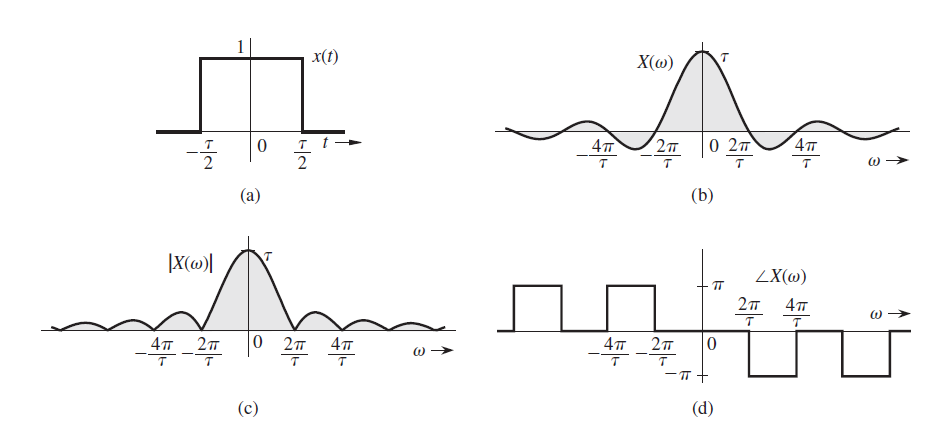
\includegraphics[width=0.78\textwidth]{rec.png}
    \end{figure}

\end{enumerate}

\subsection{Fourier Series}

\subsubsection{Fourier Series of The Delta Function}
\begin{enumerate}
  \item Note that $\delta_{T_0}(t)$ is $T_0$-periodic function, we compute its Fourier coefficients:

  \begin{equation} \label{eq:train_coeff}
    \begin{aligned}
        D_n &= \frac{1}{T_0} \int_{-\frac{T_0}{2}}^{\frac{T_0}{2}} \delta_{T_0}(t) e^{- \frac{2\pi}{T_0} i n t} dt \\
        &= \frac{1}{T_0} e^{- \frac{2\pi}{T_0} i n \cdot 0} \\
        &= \frac{1}{T_0}
    \end{aligned}
  \end{equation}
  where the second equality is by definition (sampling property) of the Dirac Delta function.

  \item We attach Figure 6.15 from B.P Lathi which contains the required plots.
    \begin{figure}[h]
        \centering
        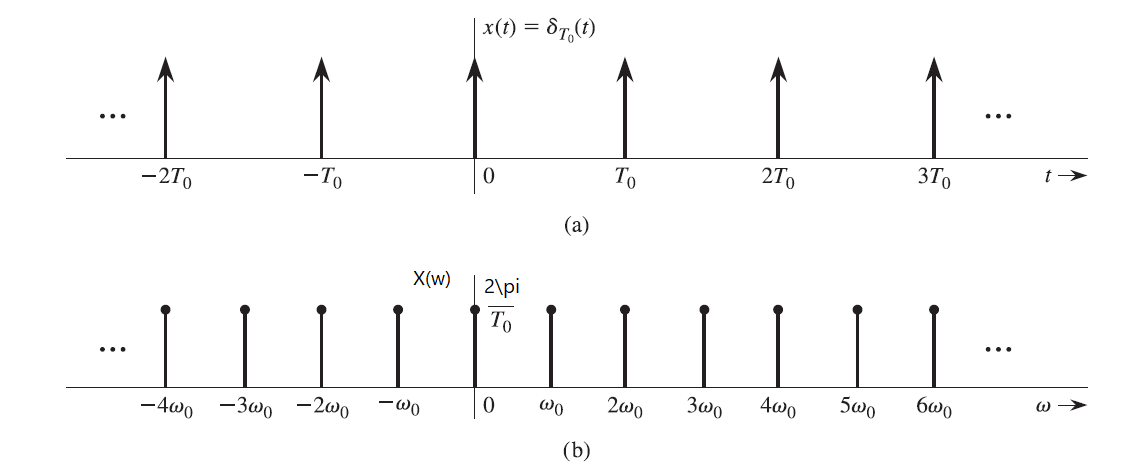
\includegraphics[width=0.78\textwidth]{train.png}
    \end{figure}

    \item $T_0$ is the period of the the impulse train given in question.

    \item Because $\delta_{T_0}(t)$ is $T_0$-periodic, we know that the frequency corresponding to the $n$-th coefficient is $\frac{2\pi}{T_0}n$
      so the interval in frequency space between $D_{n+1}$ and $D_n$ is $\frac{2\pi}{T_0}$.

\end{enumerate}

\subsection{Periodic rect Function}

Notice that by section a.5 the function $x$ drawn in the figure is the $2\pi$ periodic continuation of the function $\text{rect}\left(\frac{t}{\pi}\right) \big|_{[-\pi, \pi]}$.
As seen in class this function can be expressed as a convolution with the corresponding impulse train:
\begin{equation}
  x = \text{rect}\left(\frac{\cdot}{\pi}\right) * \delta_{2\pi}
\end{equation}

By the convolution theorem we have that
\begin{equation}
  \begin{aligned}
    \left(\mathcal{F}x\right)(\omega) &= \mathcal{F}\left( \text{rect}\left(\frac{\cdot}{\pi}\right) \right) \cdot \mathcal{F}\left(\delta_{2\pi}\right) \\
    &= \pi \, \text{sinc}\left(\frac{\pi \omega}{2}\right) \cdot \delta_{1}(\omega)
  \end{aligned}
\end{equation}
We attach Figure 6.6 from B.P Lathi which contains the amplitude plot with sign representing the phase:
\begin{figure}[h]
  \centering
  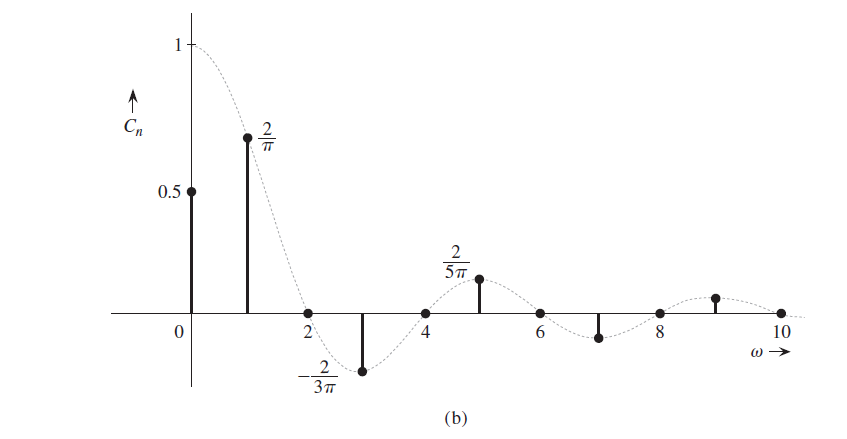
\includegraphics[width=0.78\textwidth]{sampled_sinc.png}
\end{figure}

\subsection{Heaviside Step Function}
\begin{enumerate}
  \item 
    \begin{equation}
      \begin{aligned}
        \left(\mathcal{F}x\right)(\omega) &= \int_{-\infty}^{\infty} u(\tau) e^{-a \tau -i \omega \tau} \\
        &= \int_{0}^{\infty} e^{-\left(a + i \omega\right)\tau} \\
        &= -\frac{1}{a + \omega i} \left(0 - 1\right) \\
        &= \frac{1}{a + \omega i} \\
        &= \frac{a }{a^2 + \omega^2} - \frac{\omega}{a^2 + \omega^2} i
      \end{aligned}
    \end{equation}
    
    \item For the purpose of plotting with chose $a=1$.
    \begin{figure}[h]
      \centering
      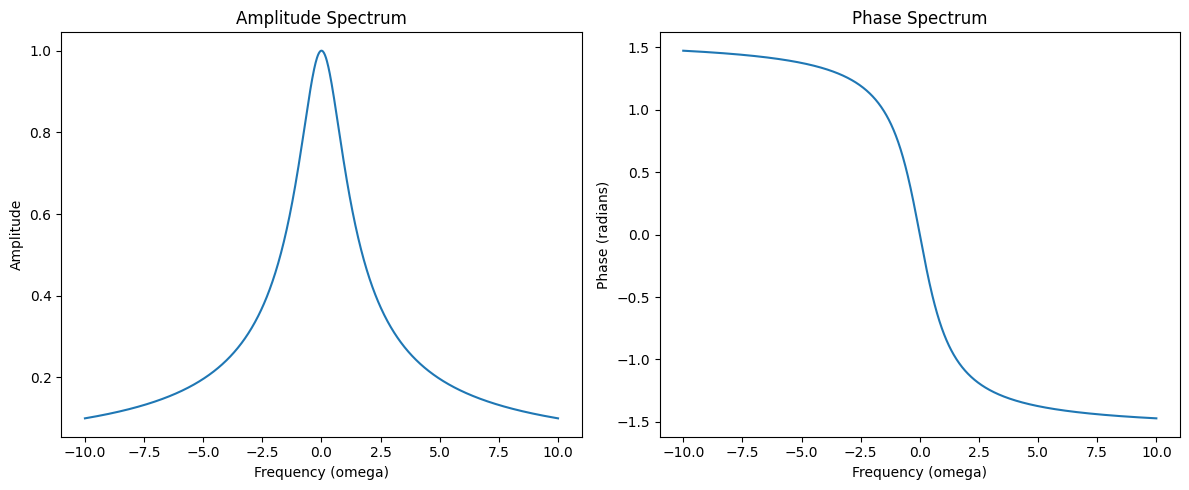
\includegraphics[width=0.9\textwidth]{from_gpt.png}
    \end{figure}

    \item Note that the amplitude spectrum of $X$ decays quadratically with the frequency, so by the convolution theorem $x$ could be used as a \textbf{low} pass filter.   
\end{enumerate}







\newpage

\section{Discrete Signals}
\subsection{Aliasing}
\begin{enumerate}
  \item The set of signals which would be aliased to 10KHz with a sampling frequency of 8KHz is given by $\sizeof{f - 10} = 8k$ for some $k\in N$.
  All such signals would be aliased to $\textbf{2KHz}$

  \item We can prevent the aliasing by passing the analog signal through an anti-aliasing filter of bandwidth 4KHz (Nyquist frequency).
  prior to sampling
\end{enumerate}

\subsection{Stereo Hearing}
When playing both channels in sync we hear the original recording.
When shifting the left track 2 ms ahead the sound appears to travel from the right ear to the left and vise versa when shifting the right track.
This occurs because when a sound source is moving relative to our ears there is a slight phase shift between the signal received in each ear.
In this case we emulate the phase shift by moving one track 2ms ahead.


\subsection{$\mathcal{Z}$ Transform}

\subsubsection{Convolution Property}
\begin{equation}
  \begin{aligned}
    \mathcal{Z}\left( x_1[n] * x_2[n] \right) &= \mathcal{Z}\left( \sum_{m \in \mathbb{Z}} x_1[m] \cdot x_2[n-m] \right) \\
    &= \sum_{n \in \mathbb{Z}} z^{-n} \sum_{m \in \mathbb{Z}} x_1[m] \cdot x_2[n-m] \\
    &= \sum_{m \in \mathbb{Z}} \sum_{n \in \mathbb{Z}} x_1[m] \cdot x_2[n-m] z^{-(n-m)} z^{-m} \\
    &= \sum_{m \in \mathbb{Z}} x_1[m] z^{-m} \sum_{n \in \mathbb{Z}} x_2[n-m] z^{-(n-m)} \\
    &= \sum_{m \in \mathbb{Z}} x_1[m] z^{-m} \sum_{n \in \mathbb{Z}} x_2[n] z^{-n} \\
    &= X_1[z] \cdot X_2[z]
  \end{aligned}
\end{equation}

\subsubsection{Time Domain Scaling}
Assuming our signal is unilateral:
\begin{equation}
  \begin{aligned}
    \mathcal{Z}\left(a^n x[n] \right) &= \sum_{n \in \mathbb{N}} a^n x[n] z^{-n} \\
    &= \sum_{n \in \mathbb{N}} x[n] \left(\frac{z}{a}\right)^{-n} \\
    &= X\left( \frac{z}{a} \right)
  \end{aligned}
\end{equation}


\subsection{DTFS}
\begin{enumerate}
  \item We compute the period of the discrete sinusoid
  \begin{equation}
    \begin{aligned}
      N_0 &= \min_{m \in \mathbb{N} \; s.t. m\left(\frac{2\pi}{0.1\pi}\right) \in \mathbb{N}} m\left(\frac{2\pi}{0.1\pi}\right)  \\
      &= 20
    \end{aligned}
  \end{equation}

  \item The sinusoid can easily be expressed as a sum of harmonic exponentials but for completeness we derive its DFTS step by step. Let us chose the 0-centered interval of length $N_0$ $S = \{-9, -8, ..., 10\}$.
  We compute the DTFS coefficients:
  \begin{equation}
    \begin{aligned}
      \mathcal{D}_r &= \frac{1}{20} \sum_{n \in S} \sin\left( 0.1\pi n \right) e^{-0.1 \pi i r n} \\
      &= \frac{1}{20} \sum_{n \in S} \frac{1}{2i} \left( e^{0.1\pi n i} - e^{-0.1\pi n i} \right) e^{-0.1 \pi i r n} \\
      &= \frac{1}{40i} \sum_{n \in S} \left( e^{0.1\pi n i \left(1-r\right)} - e^{-0.1\pi n i \left(1 + r\right)} \right) \\
      &= \frac{1}{40i} \left(\sum_{n \in S} e^{0.1\pi n i \left(1-r\right)} - \sum_{n \in S} e^{-0.1\pi n i \left(1 + r\right)} \right) \\
    \end{aligned}
  \end{equation}
  Now noticing that each sum is a geometric progression of an harmonic exponential across its period we have:
  \begin{equation}
    \mathcal{D}_r = 
    \begin{cases}
      \frac{1}{2i} &  r=1  \\
      -\frac{1}{2i} &   r=-1 \\
      0 & \text{otherwise}
   \end{cases}
  \end{equation}
  Plugging this into the DTFS we get
  \begin{equation}
    x[n] = \frac{1}{2i} \left( e^{0.1 \pi i n} +  e^{-0.1 \pi i n} \right)
  \end{equation}
\end{enumerate}

\newpage
 

\section{Technical Part}

\renewcommand{\labelenumi}{\alph{enumi}.}

\subsection{Plotting and Downsampling}
\begin{enumerate}
  \item The original sampling rate is \textbf{48 (KHz)}.
  \item There are missing timeframes in the pitch where there isn't a voiced phonation.
  \item The scipy downsampling would sound better. 
  By the Nyquist theorem naive downsampling by 2 halves the maximum frequency that can be represented.
  If our signal contains a frequency greater than $\frac{32}{2}=16$ KHz it would be aliased, disrupting the signal.
  The scipy method applies the FFT to the signal and then removes frequencies that would be aliased before resampling.
  My recording does not contain significant frequencies above 16KHz, so both methods sound similar. 
\end{enumerate}


\subsection{Spectral Noise Subtraction}

\subsubsection{Adding Noise}
Below are the 3 plots corresponding to the original (downsampled) signal, the noise and the noised signal.
\begin{figure}[h]
  \centering
  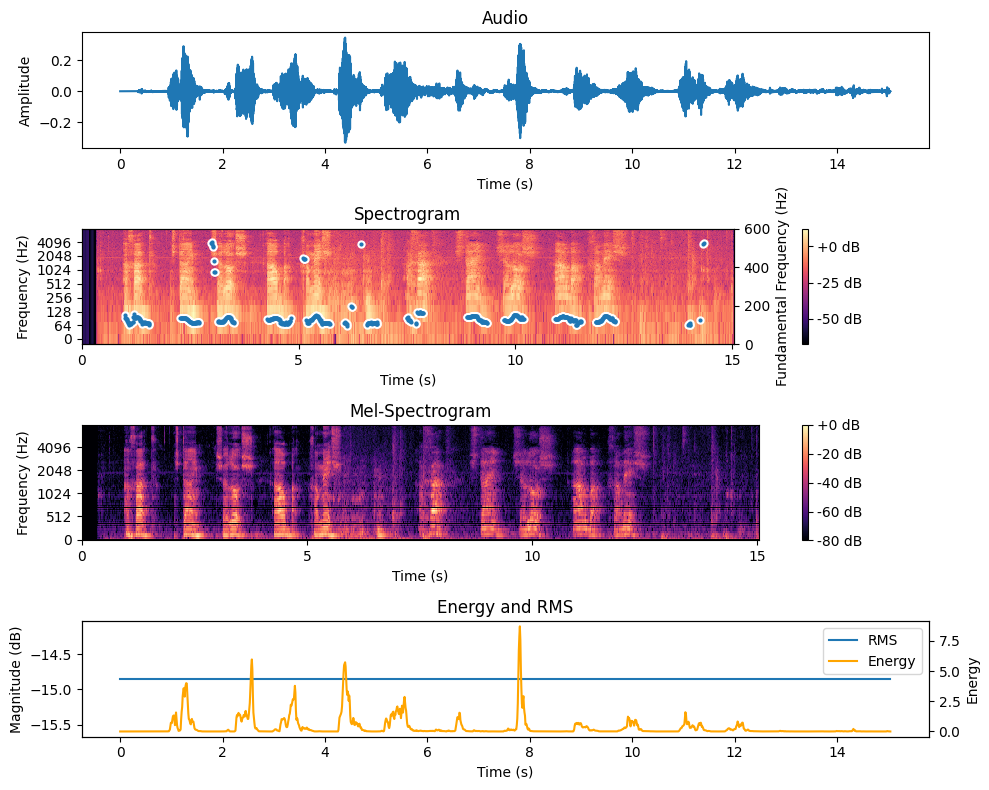
\includegraphics[width=0.9\textwidth]{downsampled_clean_plot.png}
  \caption{The clean (downsampled) signal plot.}
\end{figure}

\begin{figure}
  \centering
  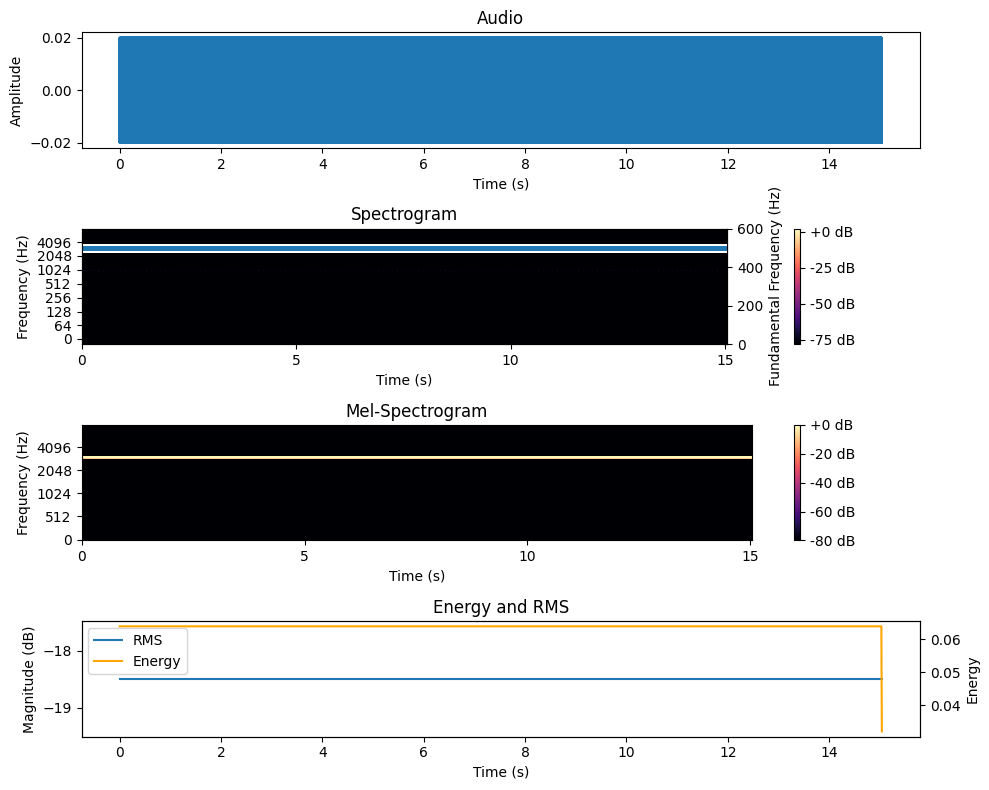
\includegraphics[width=0.9\textwidth]{noise_plot.png}
  \caption{The additive noise plot.}
\end{figure}

\begin{figure}
  \centering
  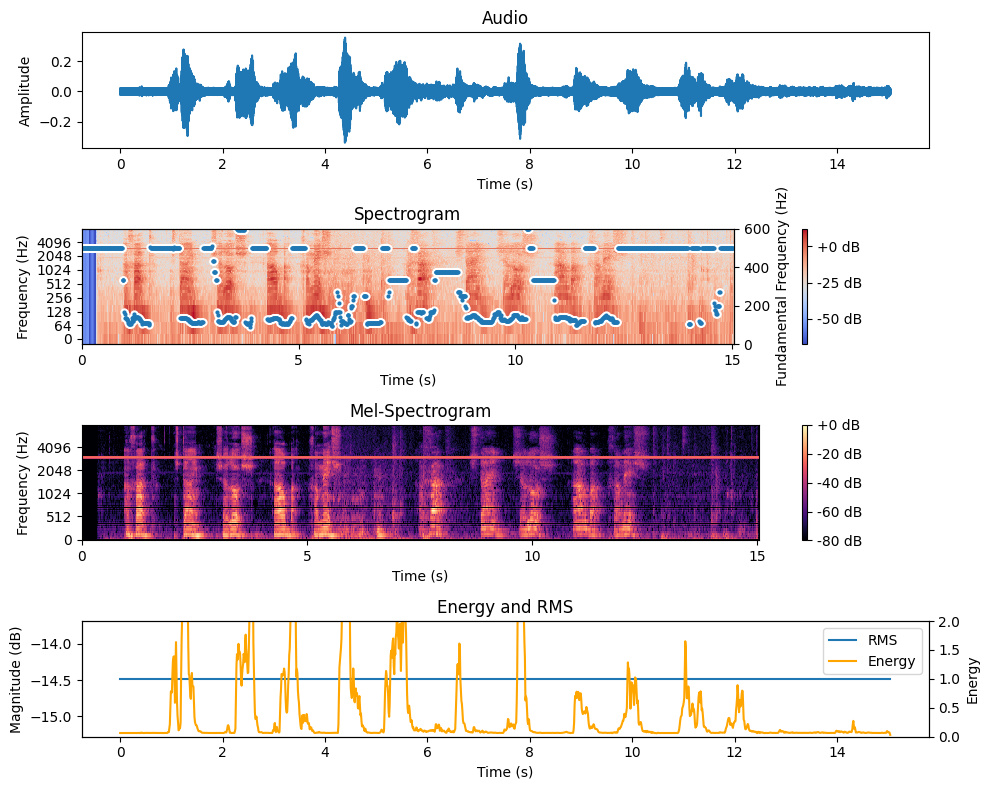
\includegraphics[width=0.9\textwidth]{noised_downsampled_plot.png}
  \caption{The noised signal plot.}
\end{figure}

\subsubsection{Spectral Substraction}
\begin{enumerate}
  \item The energy threshold plot for voice activity detection is seen in Figure 4.
  \begin{figure}
    \label{fig:VAD}
    \centering
    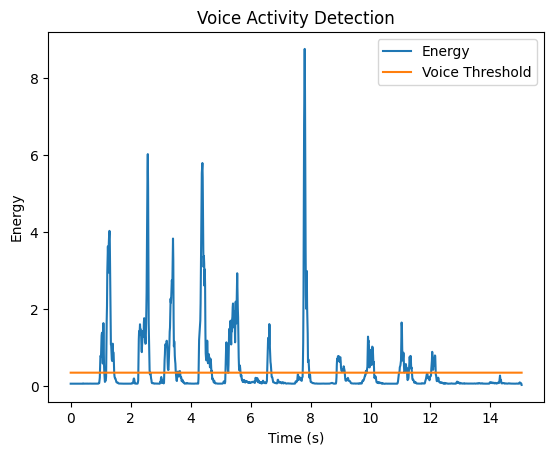
\includegraphics[width=0.64\textwidth]{voice_avctivity_detection.png}
    \caption{Energy contour plot with threshold for VAD}
  \end{figure}

  \item The plot for the denoised audio using spectral subtraction is given in Figure 5.
  \begin{figure}[b]
    \label{fig:denoised_plot}
    \centering
    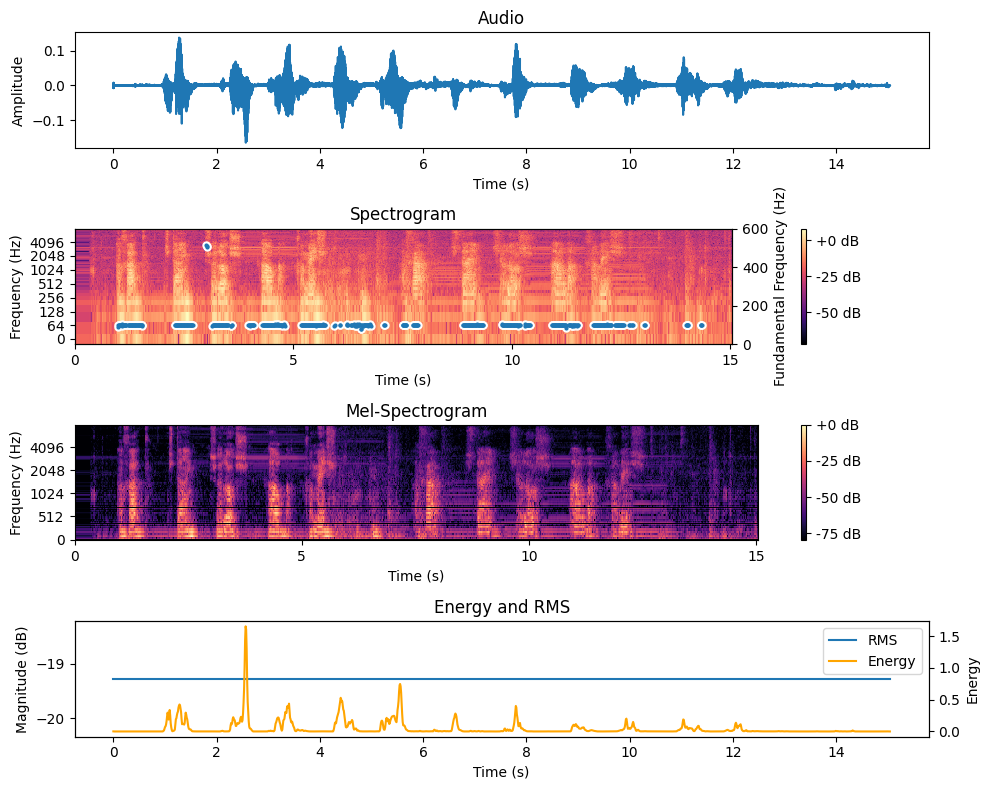
\includegraphics[width=0.9\textwidth]{cleand_audio_plot.png}
    \caption{Audio plot of the denoised signal.}
  \end{figure}
\end{enumerate}

\subsubsection{Auto Gain Control}
\begin{enumerate}
  \item The desired RMS was chosen to be \textbf{-20 dB} and the noise floor threshold was chosen to be \textbf{-46 dB}.
  Figure 6 shows the rms over time and the selected thresholds.
  \begin{figure}
    \label{fig:agc_rms}
    \centering
    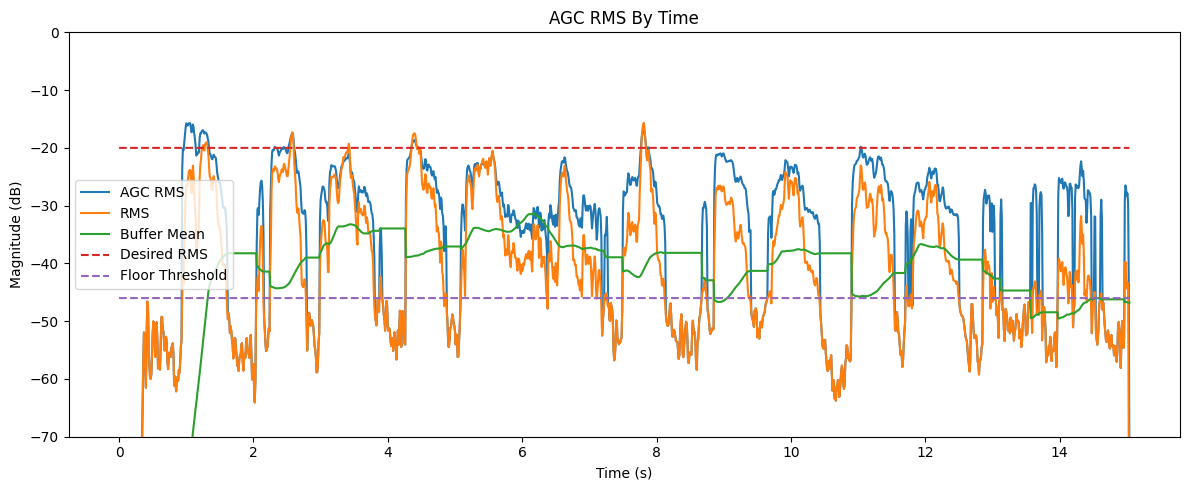
\includegraphics[width=0.9\textwidth]{agc_rms_full.png}
    \caption{RMS values for the AGC enhanced signal.}
  \end{figure}
  
  \item We plot the AGC enhanced signal in Figure 7.
  \begin{figure}
    \label{fig:agc_plot}
    \centering
    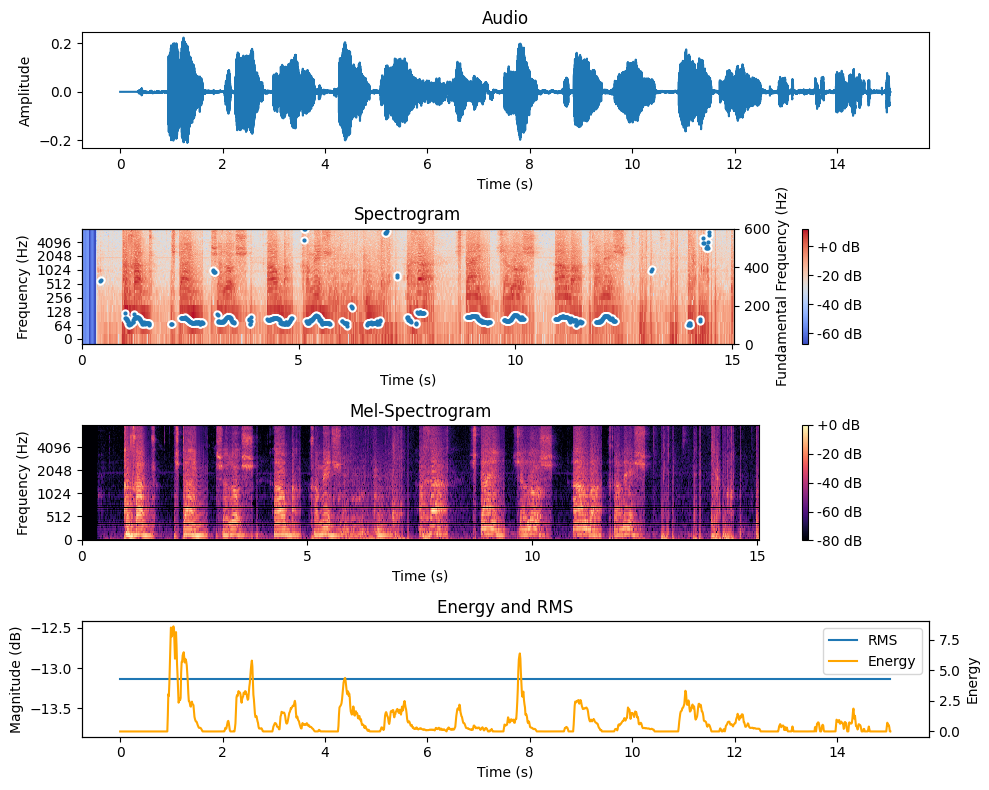
\includegraphics[width=0.9\textwidth]{agc_plot.png}
    \caption{Audio plot for the AGC enhanced signal.}
  \end{figure}

  \item The scaling factor plot is shown in Figure 8. 
  We used the metric of dB relative to reference amplitude of 1, as used in librosa.
  Note that for negative amplitude values a scaling factor lower than 1 corresponds to an increase of amplitude, a scaling factor of 1 corresponds to no change to the amplitude (such as when no voice is detected) and a factor greater than 1 corresponds to a decrease in amplitude.
  \begin{figure}
    \label{fig:scaling_factor}
    \centering
    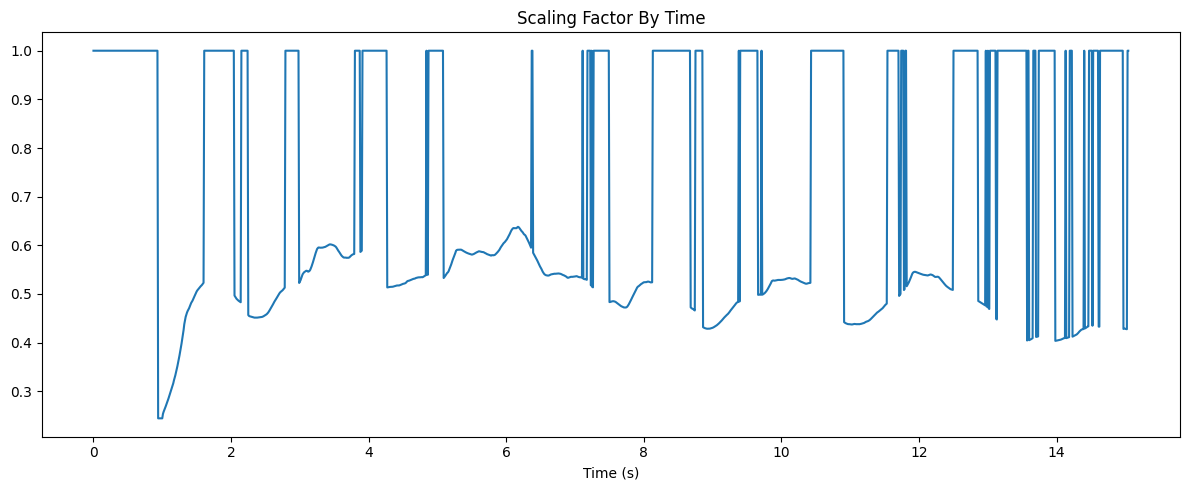
\includegraphics[width=0.9\textwidth]{agc_scaling_factor.png}
    \caption{Audio plot for the AGC enhanced signal.}
  \end{figure}

\end{enumerate}



\end{document}